
\section{Simulation}
\label{sec:simulation}

\par \noindent  With the circuit solved using the mesh and node methods, it's necesssary to solve it experimentally. In order to simulate the real conditions, which we would have encountered in the laboratory, Ngspice was used. The results obtained from this simulation will take in account the energy dissipation due to the many processes that occur such as Joule effect on conductors. Also, ngspice, when calculating the experimental results presents them with only 5 decimal cases while octave gives 6 decimal cases, resulting in a difference between the theoretical and experimental results. As such, the results will have errors associated to them (the values theoretically calculated will differ from these) which can and will be calculated so that conclusions can be taken from the experiment. Using this software, we were able to verify the results obtained from the methods already described. 
\par \noindent  In order to describe the circuit to be studied, it is necessary to follow some guidelines. Firstly, it was needed to specify , for each component, which were its positive and negative nodes. Because of that, the current directions were defined accordingly to the ones seen in the picture describing the mesh and node methods. As such, the electric resistances and current sources are going to have the positive node in the location of the current input and the negative node in the current output. The voltage sources nodes were defined so that the nodes are in accordance with the pre established nodes.
\par \noindent Apart from this, it was also necessary to establish the values of the resistance, current and voltage associated with the resistors and independent current and voltage sources. The dependent sources, Vc and Ib (Hc and Gb in ngspice beacuse of the symbolic representation in the program), were respectively current controlled voltage source and voltage controlled current source. Because of that, kc and kb were in kOhm and mS as the script indicated. In the case of Vc, it was needed to indicate a control voltage source, Ve which, even though it doesn't exist, is going to measure the current Ic, the control current, passing through it. This voltage control has a null potential which means that the current flowing before reaching this component is going to be the same coming out of it, allowing us to measure the current. The nodes of Ve were placed in the circuit so that the current input is in the positive node of the voltage source and the outup of the current is in the negative node of the source.  In the case of Ib, it was needed to introduce the nodes in which the potential difference is going to be read (again the positive node in first place and then the negative one).
\par \noindent In the picture below, a brief representation of the interpertation of the circuit by the ngspice programme is presented.

\begin{figure}[h]
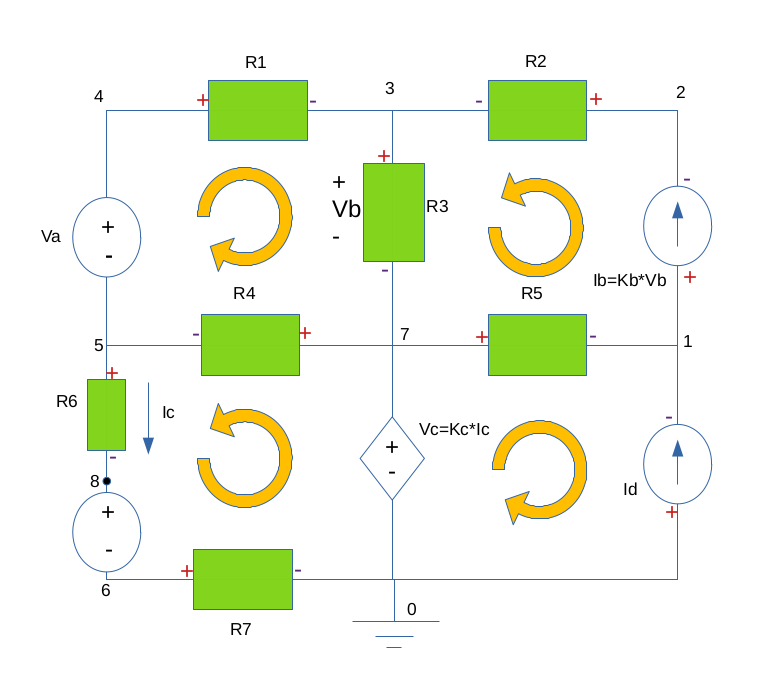
\includegraphics[width=0.5\textwidth]{Esquema_salito.PNG}
\centering
\caption{Circuit with voltage control source - current flow and voltage difference representation}
\label{fig:figure5}
\end{figure}

\par \noindent Finally, a table with the values obtained is asked every time the programme is run, in order to obtain the looked for data as we can see below. 
\vspace{5mm}
\begin{table}
\centering
\begin{tabularx}{0.8\textwidth} {
  | >{\raggedright\arraybackslash}X
  | >{\raggedleft\arraybackslash}X | }
 \hline
@cb[i] & 0.000000e+00\\ \hline
@ce[i] & 0.000000e+00\\ \hline
@q1[ib] & 7.022567e-05\\ \hline
@q1[ic] & 1.404513e-02\\ \hline
@q1[ie] & -1.41154e-02\\ \hline
@q1[is] & 5.765392e-12\\ \hline
@rc[i] & 1.411536e-02\\ \hline
@re[i] & 1.411536e-02\\ \hline
@rf[i] & 7.022567e-05\\ \hline
@rs[i] & 0.000000e+00\\ \hline
v(1) & 0.000000e+00\\ \hline
v(2) & 0.000000e+00\\ \hline
base & 2.254108e+00\\ \hline
coll & 5.765392e+00\\ \hline
emit & 1.411536e+00\\ \hline
vcc & 1.000000e+01\\ \hline

\end{tabularx}
\end{table}




